Una vez establecido el objetivo de este proyecto en la introducción, en este capítulo se describirán los conceptos generales necesarios para la comprensión de este documento. Para ello, en primer lugar se detalla el proceso de onboarding en proyectos software y las dificultades que presenta, junto con el trabajo previo realizado en este ámbito.

Por otro lado, se explicará a grandes rasgos qué son los agentes basados en grandes modelos de lenguaje (\textit{Large Language Models}), su funcionamiento e interacción con herramientas externas. Se introduce además el Model Context Protocol como estándar de comunicación entre estos componentes.


Finalmente, se aborda el estado del arte en arquitecturas de agentes, sus aplicaciones en proyectos software, técnicas de evaluación y varias consideraciones sobre el ajuste de estos.

\section{Onboarding en proyectos software}
El proceso de incorporación de nuevos desarrolladores de software constituye un desafío persistente para las organizaciones tecnológicas, donde los recién incorporados se enfrentan a una sobrecarga informativa mientras los desarrolladores senior ven afectada su productividad al destinar tiempo considerable a actividades de formación y mentoría \cite{sim_ramp-up_1998}. 

Si bien prácticas como la designación de mentores han demostrado ser efectivas para facilitar la integración de nuevos miembros, estas incrementan significativamente la carga de trabajo sobre los profesionales experimentados, generando potenciales retrasos en los proyectos \cite{steinmacher_systematic_2015}.

En este contexto, los modelos de lenguaje de gran escala emergen como una alternativa prometedora para transformar el proceso de onboarding. Su capacidad para sintetizar y razonar sobre una cantidad de información cada vez mayor ofrece la promesa de una orientación personalizada e instantánea que podría reducir la dependencia de los desarrolladores senior, preservar la productividad global de los equipos, y facilitar una incorporación más eficiente \cite{ritz_artificial_2023}.

\subsection{Trabajo previo}
\label{sec:trabajo_previo}

La Universidad del País Vasco, en colaboración con LKS Next, desarrolló el prototipo denominado I Need a Hero (INAH), diseñado para aprovechar el potencial de los LLM en la localización de expertos dentro de la organización \cite{azanza_can_2024}. INAH opera en dos fases: primero crea perfiles de ``héroes'' extrayendo información de currículos de empleados dispuestos a asistir; luego, ante una consulta, utiliza GPT-3.5 para identificar las competencias requeridas y localizar a los profesionales que las poseen.

En una línea de estudio complementaria, un trabajo reciente ha presentado el sistema ``Onboarding Buddy'', el cual implementa una arquitectura multiagente que organiza diversos componentes especializados para proporcionar asistencia contextualizada durante la incorporación de nuevos desarrolladores \cite{ionescu_multi-agent_2025}. El sistema fundamenta su funcionamiento en la generación dinámica de planes mediante cadena de pensamiento \ref{plani}, evaluados posteriormente para determinar su posible descomposición en sub-tareas procesadas en paralelo por otros agentes.

Aunque las investigaciones anteriores han demostrado el potencial de los agentes en este ámbito, dichas propuestas se limitan a obtener información de una única fuente de datos. Por tanto, el presente trabajo pretende explorar el potencial de dichos sistemas en escenarios similares a entornos productivos, donde la información se encuentra distribuida entre múltiples fuentes.

\section{Agentes de Grandes Modelos de Lenguaje (LLM)}

Los agentes de Inteligencia Artificial son programas informáticos que implementan modelos computacionales para ejecutar diversas funciones específicas del contexto en el que se aplican. Tras siete décadas y media de investigación, los esfuerzos en el campo se han focalizado en agentes basados en grandes modelos de lenguaje. 

\subsection{Modelos LLM}

Los Grandes Modelos de Lenguaje son redes neuronales especializadas en el procesamiento del lenguaje natural que funcionan mediante un mecanismo de entrada-salida de tokens \ref{token}. Estos modelos reciben secuencias de tokens como entrada, denominada comúnmente "\textit{prompt}", y generan secuencias de tokens como salida, aplicando durante este proceso las representaciones y relaciones semánticas aprendidas durante su fase de entrenamiento con extensos corpus textuales  \cite{vaswani_attention_2023}.

Para comprender el funcionamiento de estos agentes, resulta imprescindible asimilar previamente conceptos como la tokenización, las representaciones vectoriales del lenguaje y el ajuste de dichos modelos.

\paragraph{Tokens}\label{token}
Los tokens constituyen la unidad mínima de texto que el modelo puede procesar. Dado que dichos modelos operan sobre estructuras matemáticas, requieren transformar el lenguaje natural en representaciones matriciales. Para lograr esta conversión, el texto se segmenta en dichas unidades mínimas, que pueden corresponder a caracteres individuales, fragmentos de texto o palabras completas. El conjunto íntegro de estas unidades reconocibles por el modelo configura su vocabulario. 

\paragraph{Representaciones vectoriales}
Constituyen vectores numéricos de dimensionalidad fija que codifican la semántica inherente a cada token. Por ejemplo, una dimensión específica podría especializarse en representar conceptos abstractos. En este contexto, la representación vectorial del token ``animal'' contendría un valor más elevado en dicha dimensión que la correspondiente al término ``gato'', reflejando su mayor grado de abstracción conceptual.

\paragraph{Ajuste de modelos instruct}
El entrenamiento de los LLM (véase Anexo \ref{anexo:entrenamiento_redes}) se estructura en dos fases diferenciadas. La primera corresponde al preentrenamiento, donde el modelo procesa extensos conjunto de datos textuales con operaciones como intentar predecir el siguiente token en la secuencia. Esta fase permite al modelo captar las complejas estructuras sintácticas y relaciones semánticas inherentes al lenguaje natural. La segunda fase consiste en el ajuste fino, donde el modelo previamente entrenado se especializa mediante conjuntos de datos específicos y etiquetados (consulte Anexo \ref{anexo:datos_et}), optimizando su capacidad para ejecutar tareas concretas de clasificación o generación de texto.

Los agentes basados en LLM implementan en su mayoría modelos \textit{instruct}, variantes especialmente ajustadas para responder a consultas e instrucciones de usuarios. Dentro de esta categoría se encuentran GPT (base de ChatGPT\footnote{ChatGPT:\url{https://chatgpt.com}}) de OpenAI\footnote{OpenAI:\url{https://openai.com/}}, Claude Sonnet de Anthropic\footnote{Anthropic:\url{https://www.anthropic.com/}}, y LLama-Instruct de Meta\footnote{Meta: \url{https://about.meta.com/es/}}.



\subsection{Interacción con herramientas externas}
Los agentes LLM poseen la capacidad de interactuar con diversas herramientas como búsquedas web, bases de datos o interfaces de usuario. Fundamentalmente, este tipo de modelos solo genera tokens de texto, por lo que la integración de herramientas se implementa mediante palabras clave o tokens especiales que este puede incluir en su salida. Para ello, en el texto de entrada se especifica el esquema de la función a utilizar y, si decide emplearla, el modelo generará el texto correspondiente. Posteriormente, se procesa la respuesta para extraer llamadas a funciones si las hubiese.

La interacción con herramientas sigue un patrón secuencial. Tras realizar la llamada a la herramienta, la salida de esta se utilizará como entrada para el siguiente mensaje del modelo. La Figura \ref{fig:herramientas} ilustra el esquema de un agente con acceso a una API del clima que consulta información meteorológica. Como el modelo carece de dicha información en tiempo real, se le indica en el prompt la posibilidad de invocar esta función. Al incluir la llamada en su texto de salida, se ejecuta la función y su respuesta se transmite al modelo para generar el resultado final.

\begin{figure}[H]
  \centering
  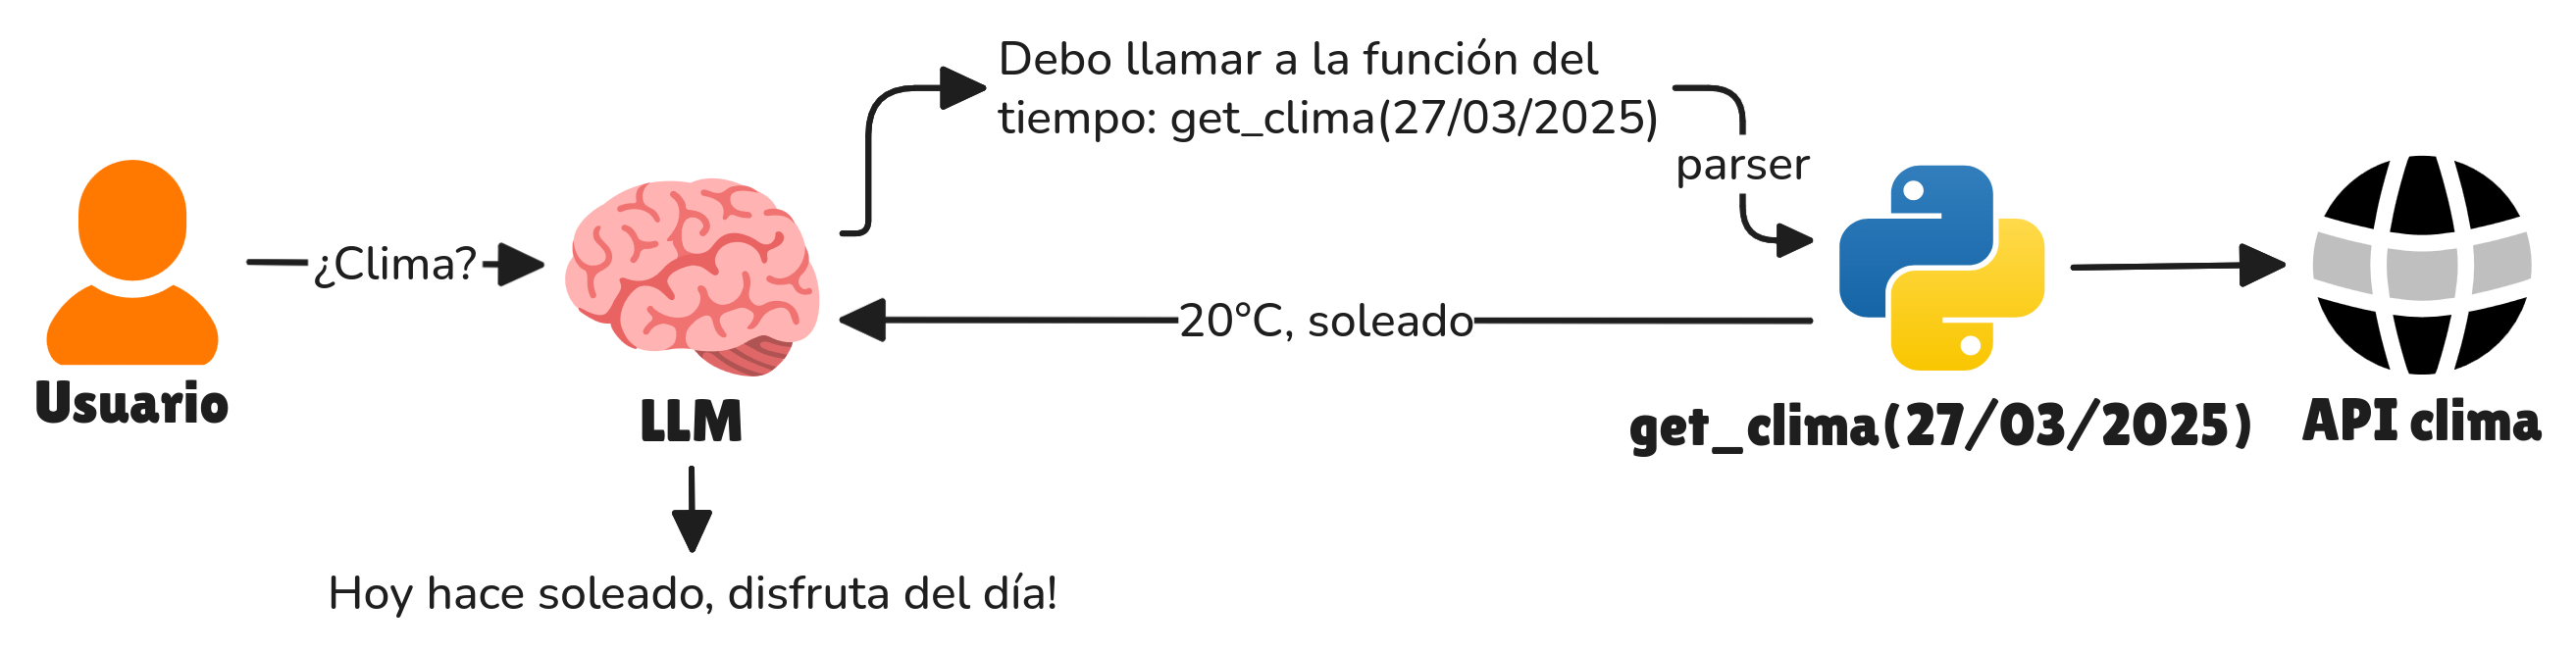
\includegraphics[width=1.05\linewidth]{figures/herramienta.png}
  \caption{Ejemplo de interacción de un modelo LLM con una herramienta externa.}
  \label{fig:herramientas}
\end{figure}


\subsubsection{Patrón ReAct}
\label{sec:react}
El agente Reasoning and Act (ReAct) constituye uno de los patrones más utilizados \cite{yao_react_2023}. Se basa en un ciclo de tres pasos fundamentales: el razonamiento como generación de pensamiento sobre posibles acciones, la acción como ejecución de la herramienta seleccionada y la observación como procesamiento del resultado obtenido. Este ciclo se repite iterativamente hasta que durante la fase de razonamiento se determina que la tarea ha sido completada.

%xu_rewoo_2023 -> rewoo para no pasar observaciones a react ~orquestar
%react todo
%wang_executable_2024 -> tools con código, igual mejor donde herramientas?



\subsection{Abstracciones en frameworks}
\label{sec:abst}
En pleno auge de los agentes LLM, surgen cada vez más bibliotecas y frameworks que estandarizan su implementación. Estos marcos de trabajo ofrecen abstracciones de alto nivel para reutilizar funcionalidades comunes presentes en la mayoría de sistemas de agentes.
Las principales funcionalidades proporcionadas son las siguientes: 
\begin{itemize}
\item {\textbf{Gestión de modelos:}} la ejecución de modelos de lenguaje requiere del dominio de estos, ya que cada uno posee tokenizadores (véase Anexo \ref{anexo:tokenizer}) específicos y esquemas propios de entrada y salida. Los frameworks ofrecen interfaces unificadas, facilitando el uso de diversos modelos sin necesidad de conocimientos técnicos excesivamente detallados.
\item {\textbf{Interacción conversacional:}} la comunicación con los agentes se efectúa mediante un esquema conversacional, donde el modelo recibe un texto de entrada y genera una respuesta correspondiente. Las respuestas y entradas se concatenan secuencialmente para preservar el contexto de la conversación, cada consulta subsiguiente incorpora todos los intercambios precedentes.
\item {\textbf{Uso de herramientas externas:}} toda la complejidad de la interacción se abstrae en el framework, por lo que el desarrollador únicamente debe especificar la función que desea incorporar.
\item {\textbf{Interacción entre agentes:}} los agentes pueden establecer comunicación entre sí, permitiendo la construcción de sistemas con mayor complejidad. Algunos frameworks establecen protocolos que definen las modalidades de comunicación entre los distintos agentes.
\end{itemize}

Para este trabajo utilizaremos LangChain para la gestión de llamadas a APIs de modelos y prompting, LangGraph para la orquestación de flujos agénticos, y LangSmith para el seguimiento de trazas de llamadas a modelos y herramientas, así como para la ejecución de las evaluaciones del sistema. Para la gestión de los conjuntos de datos y entrenamiento de modelos utilizaremos HuggingFace.\footnote{HuggingFace: \url{https://huggingface.co/}}

\section{Model Context Protocol (MCP)}
\label{sec:mcp_prots}
El protocolo MCP, desarrollado por Anthropic, estandariza la comunicación entre agentes LLM y herramientas. Permite que aplicaciones diversas ofrezcan herramientas a agentes externos sin exponer detalles de implementación \cite{noauthor_model_nodate}.

La Figura \ref{fig:mcp} ilustra el esquema operativo del protocolo. En este ejemplo, los desarrolladores de Jira\footnote{Jira: \url{https://www.atlassian.com/es/software/jira}} y GitHub\footnote{GitHub: \url{https://github.com/}} han implementado un servidor MCP que traduce las interacciones con sus APIs y proporciona herramientas al cliente MCP. Esto permite que el desarrollador del agente se enfoque exclusivamente en conectar las herramientas del cliente con el agente, sin necesidad de interactuar con APIs externas. Asimismo, el cliente MCP gestiona la comunicación entre servidores, facilitando al agente el acceso directo a múltiples herramientas.

\begin{figure}[h]
  \centering
  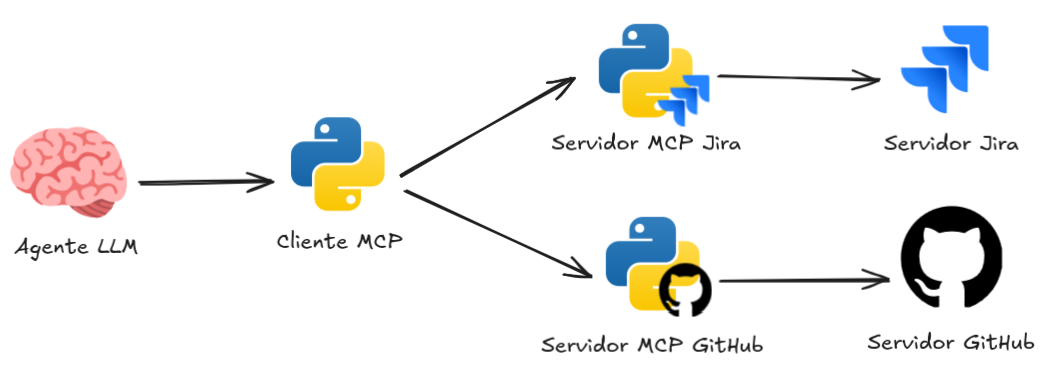
\includegraphics[width=1\linewidth]{figures/mcp.png}
  \caption{Esquema de funcionamiento del Model Context Protocol.}
  \label{fig:mcp}
\end{figure}


El protocolo ofrece dos modos de operación para establecer la comunicación entre cliente y servidor:
\begin{itemize}
  \item{\textbf{Comunicación SSE: } el protocolo \textit{Server-Sent Events} (SSE) establece un canal de comunicación unidireccional sobre HTTP desde el servidor hacia el cliente, proporciona actualizaciones en tiempo real con capacidad de streaming. En el protocolo MCP, el cliente efectúa solicitudes para la ejecución de herramientas en el servidor mediante HTTP, a lo que el servidor puede responder mediante eventos SSE.}
\item{\textbf{Comunicación STDIO: } el protocolo de entrada y salida estándar (STDIO) facilita la comunicación bidireccional entre cliente y servidor a nivel de proceso en el sistema operativo. Este mecanismo permite el intercambio de información en formato JSON a través de los canales estándar del sistema. Su diseño, orientado principalmente a entornos locales, restringe la conexión a un único cliente por servidor al limitarse a la comunicación entre dos procesos.}
\end{itemize}
La aplicación Claude Desktop\footnote{Claude Desktop: \url{https://claude.ai/download}} de Anthropic demuestra el potencial del protocolo. Esta plataforma permite integrar servidores MCP de terceros con configuración mínima mediante gestores de paquetes estándar, facilitando el acceso a múltiples herramientas en la interfaz de chat.

\section{Estado del arte en arquitecturas de agentes LLM}
\label{sec:estado_arte}

La comunidad científica ha diseñado diversas arquitecturas de agentes para optimizar el rendimiento de los modelos disponibles. La arquitectura RAG se distingue por complementar la entrada del modelo con información recuperada de documentos relevantes. Otras propuestas se centran en mejorar la comunicación y coordinación entre agentes.

\subsection{Arquitectura RAG}

Los modelos LLM poseen un conocimiento restringido a los datos con los que fueron entrenados. Para superar esta limitación, el enfoque RAG (Retrieval-Augmented Generation) complementa la generación del LLM mediante la recuperación de información relevante desde repositorios de conocimiento externos. La Figura \ref{fig:rag} ilustra un ejemplo de su funcionamiento.    

\begin{figure}[hbtp]
  \centering
  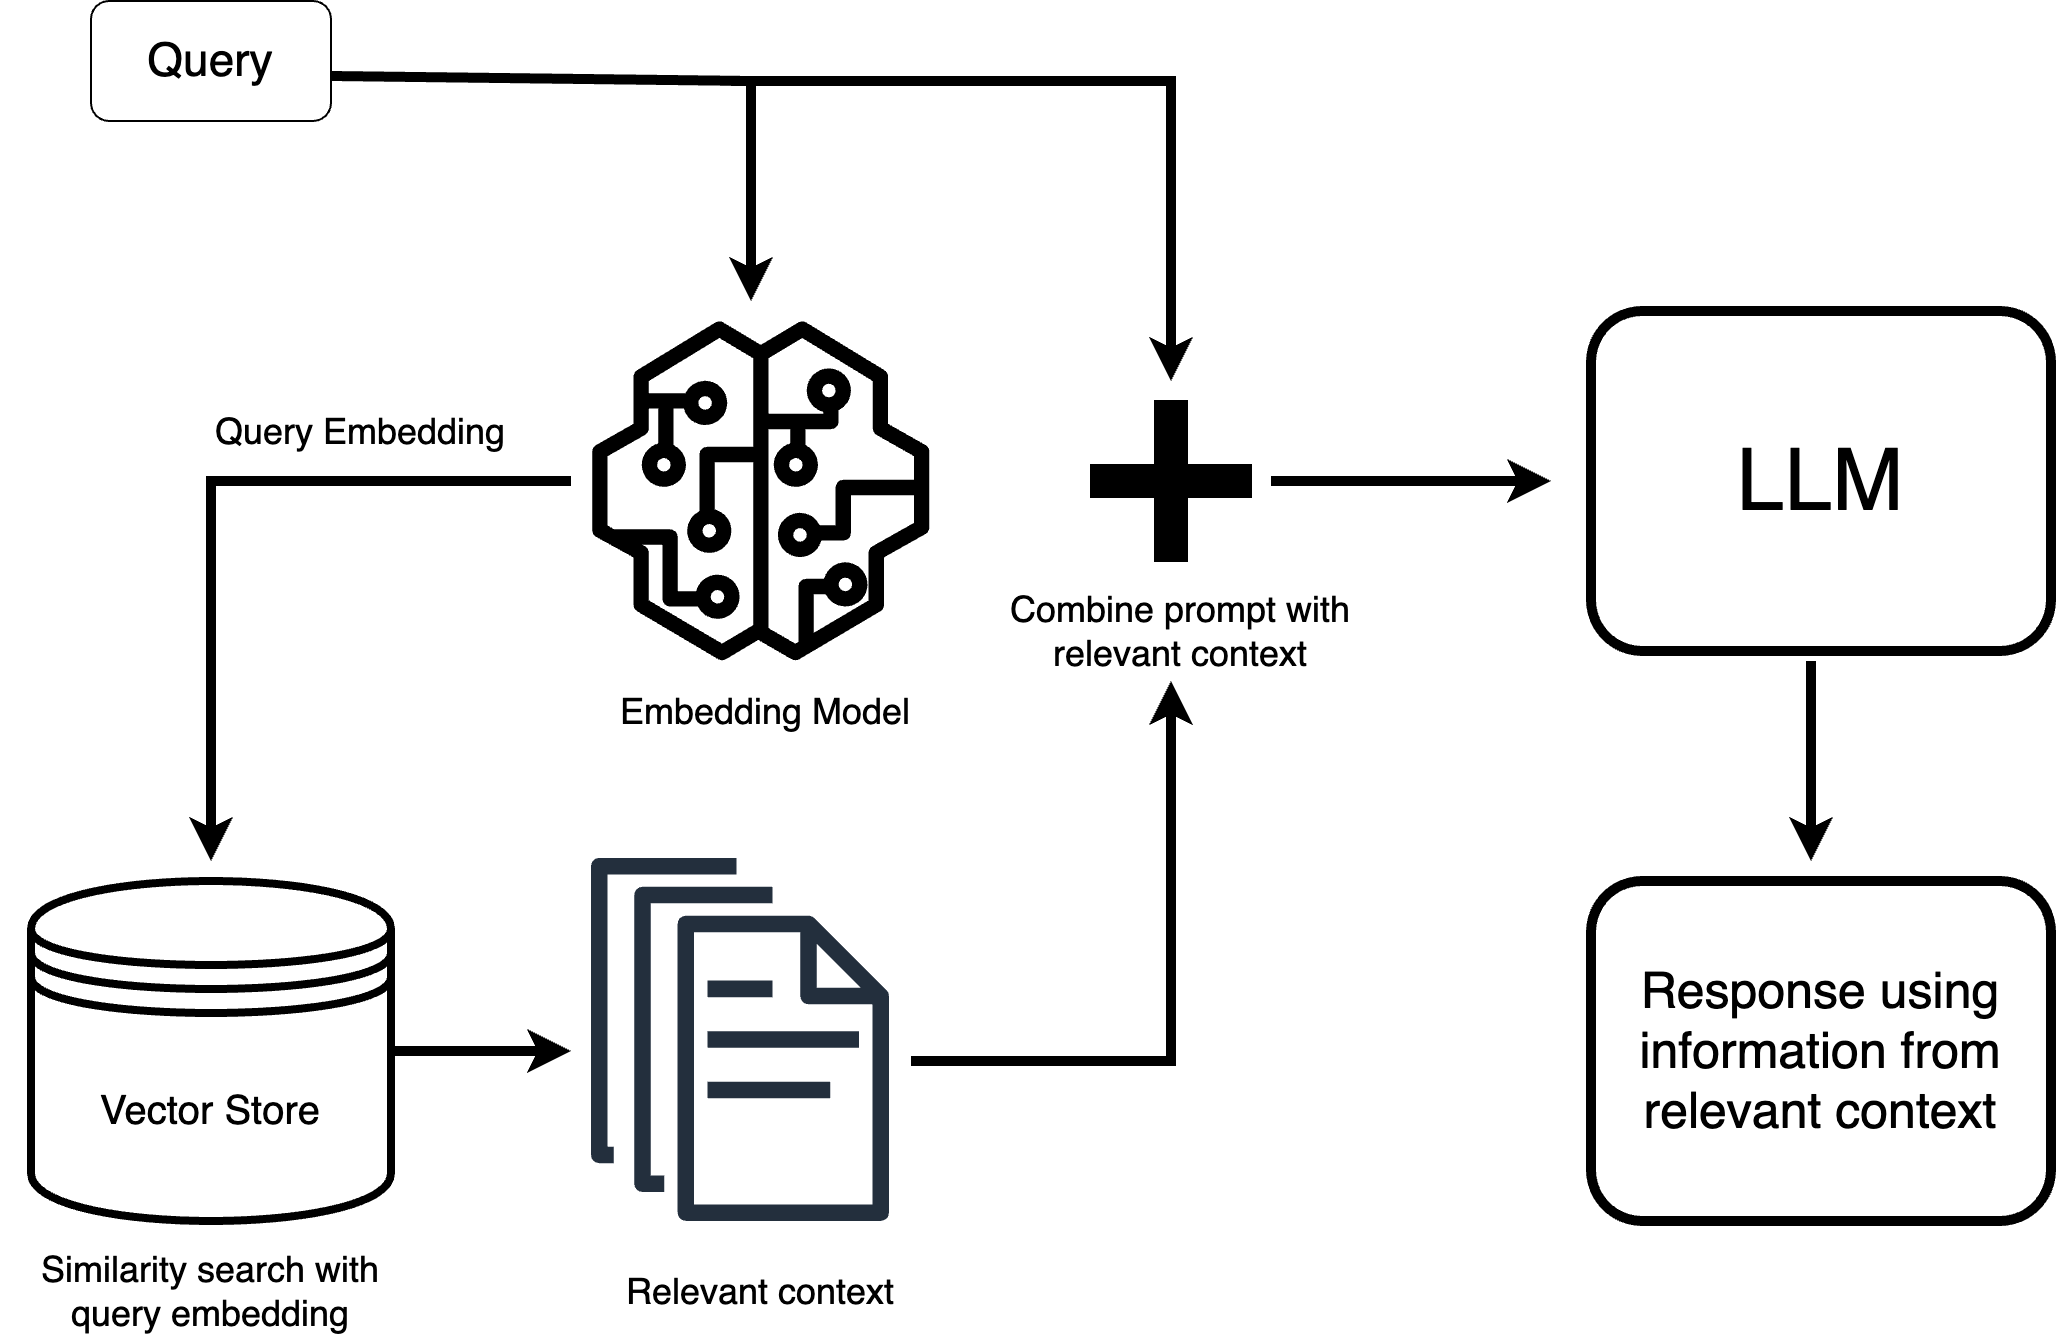
\includegraphics[width=0.75\linewidth]{figures/RAG.png}
  \caption{Esquema de funcionamiento de la arquitectura RAG en un LLM \href{https://www.clarifai.com/blog/what-is-rag-retrieval-augmented-generation}{Fuente}.}
  \label{fig:rag}
\end{figure}

La recuperación de documentos relevantes se puede implementar mediate recuperadores dispersos: expresiones regulares, búsqueda de n-gramas, palabras clave, entre otras. No obstante, el enfoque predominante consiste en el uso de recuperadores densos \cite{gao_retrieval-augmented_2024}, conocidos como indexación vectorial. En este método, los documentos se transforman en vectores, generalmente mediante LLMs especializados en codificación, denominados \textit{embedders}. Al representar los documentos en un espacio vectorial, es posible recuperar aquellos semánticamente más pertinentes mediante la comparación del vector de consulta con los vectores de los documentos indexados, utilizando métricas como la distancia coseno (definida en Anexo \ref{anexo:dis_cos}).

\subsubsection{Estrategias RAG avanzadas}
\label{sec:estr_rag}
La optimización del rendimiento en arquitecturas RAG ha sido ampliamente estudiada \cite{zhu_retrieving_2021, gao_retrieval-augmented_2024}, enfocándose en tres áreas principales: el procesado de documentos, los sistemas de recuperación y la mejora del flujo de generación.

Dentro del procesado de documentos, la ventana solapada (Figura \ref{fig:rag_1}) superpone fragmentos de texto al dividir documentos largos en segmentos indexables para evitar pérdida de información en los límites entre fragmentos. En cuanto a la mejora del flujo de generación, los sistemas de salto múltiple (Figura \ref{fig:rag_2}) alternan entre recuperación y generación para abordar tareas complejas \cite{khattab_demonstrate-search-predict_2023, shao_enhancing_2023, qi_answering_2021, zheng_take_2024, trivedi_interleaving_2023}.

\begin{figure}[h]
\centering
\makebox[\textwidth][c]{%
  \subfloat[Ventana solapada para segmentación\label{fig:rag_1}]{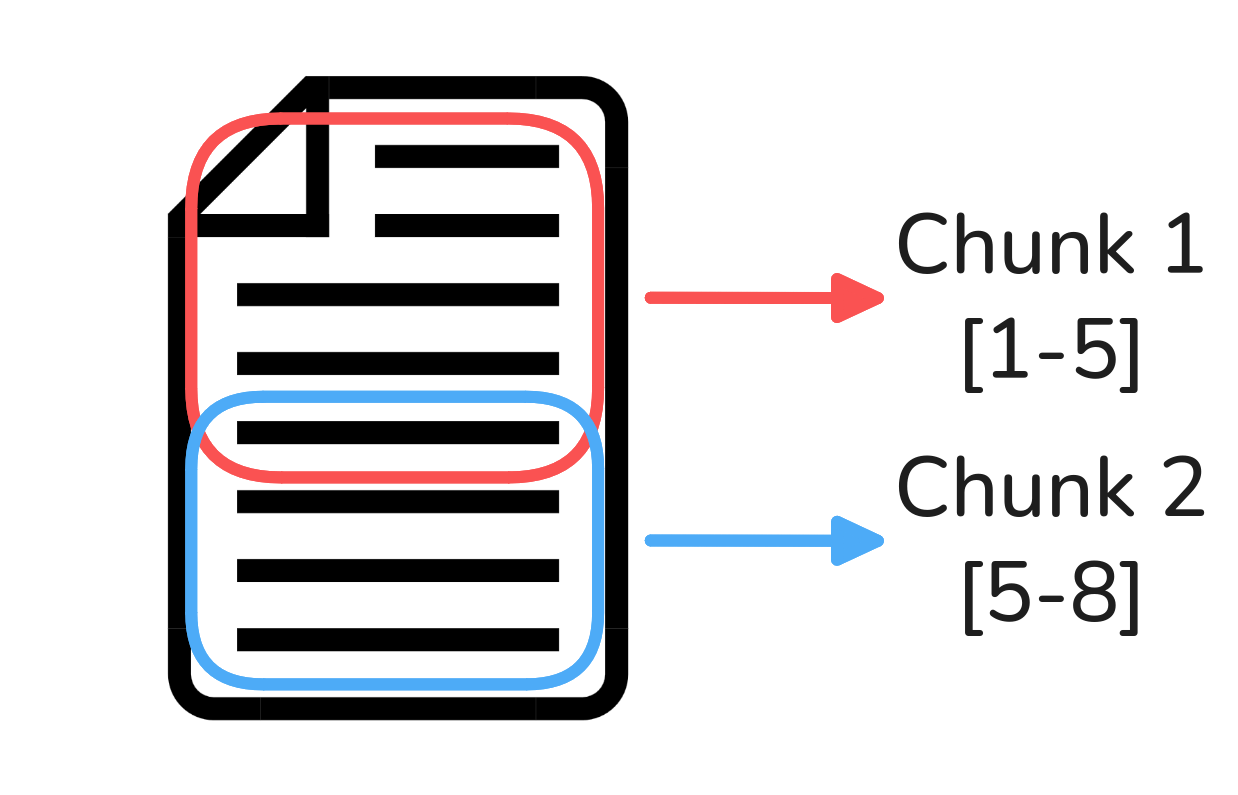
\includegraphics[width=0.35\textwidth]{figures/overlap.png}}
  \hfill
  \subfloat[Iteración de recuperación y generación mediante RAG\label{fig:rag_2}]{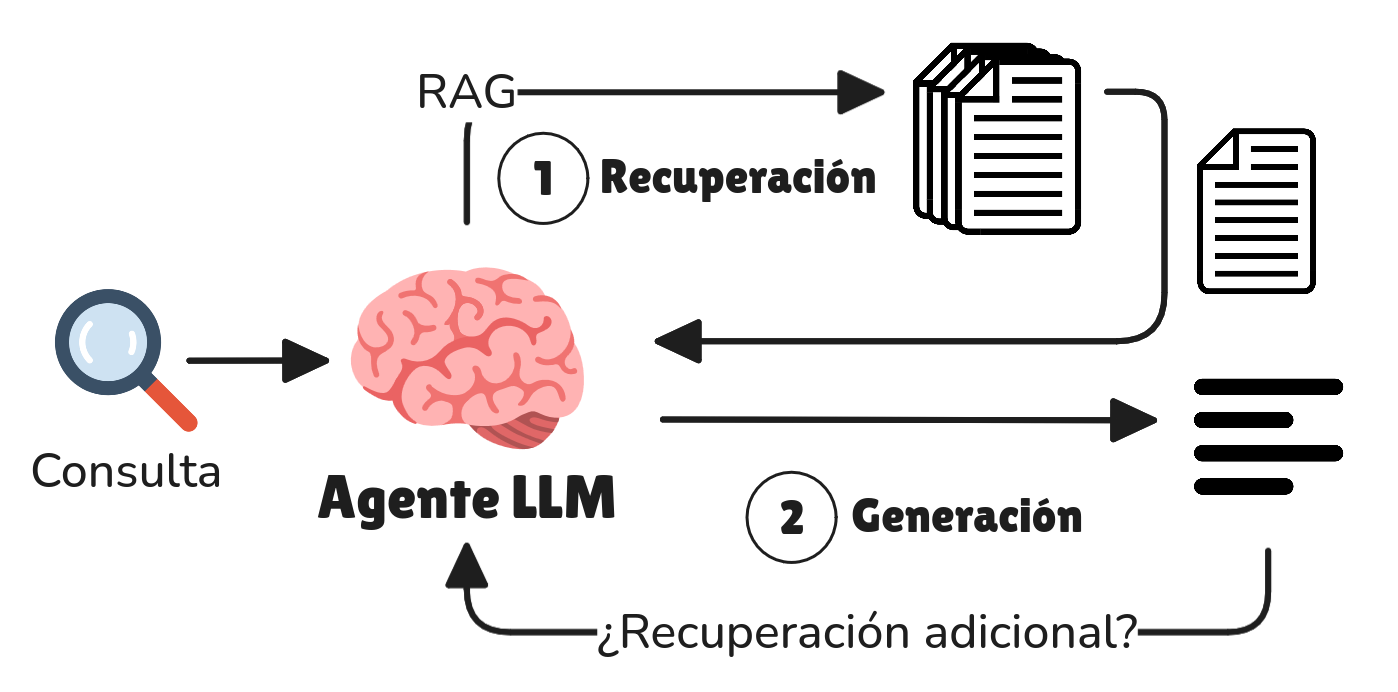
\includegraphics[width=0.75\textwidth]{figures/multihop.png}}
}
\caption{Técnicas avanzadas de RAG}
\label{fig:rag_avanzado}
\end{figure}


\subsection{Arquitecturas de interacción entre agentes}
La interacción entre agentes LLM constituye un campo de investigación activo, distinguiéndose diversos avances en módulos de memoria, planificación e interacción multiagente \cite{wang_survey_2024}.
\begin{itemize}
  \label{sec:modulos_memoria}
  \item{\textbf{Módulos de memoria}}: en una interacción conversacional, el modelo procesa todos los mensajes previos, pudiendo generar un contexto excesivamente amplio. Para mitigar este problema, se han desarrollados módulos de memoria que almacenan información relevante de interacciones pasadas de forma resumida \cite{zhang_building_2024-1, fischer_reflective_2023, liang_unleashing_2023}. Esta memoria puede consultarse posteriormente mediante RAG, permitiendo recuperar los elementos más relevantes según el contexto \cite{zhao_expel_2024}.

Algunos módulos se inspiran en la estructura de la memoria humana \cite{zhong_memorybank_2024}, incorporando mecanismos que almacenan información con distintas temporalidades y niveles de relevancia \cite{wang_survey_2024, park_generative_2023}.


\item{\textbf{Planificación}}\label{plani}: los mecanismos de planificación potencian el razonamiento de los agentes sobre sus acciones futuras.

  Entre estos mecanismos destaca el prompting de cadena de pensamiento (Chain of Thought) \cite{wei_chain--thought_2023}, que instruye al modelo para elaborar un razonamiento secuencial previo a su decisión final, permitiendo así descomponer problemas complejos paso a paso.
Partiendo de este enfoque, estrategias avanzadas como la autoconsciencia \cite{liang_unleashing_2023} lo amplían mediante la generación de múltiples cadenas de razonamiento independientes y la posterior selección de la respuesta óptima entre ellas \cite{yao_tree_nodate, wang_recmind_2024}. De manera complementaria, las técnicas de reflexión \cite{shinn_reflexion_nodate, madaan_self-refine_nodate, miao_selfcheck_2023} implementan un proceso iterativo donde el propio modelo evalúa y refina sus respuestas.

Por otro lado, la estructuración de acciones constituye una metodología ampliamente adoptada en la planificación \cite{lin_swiftsage_nodate, huang_language_nodate, wang_describe_2024}. Esta técnica permite definir planes de alto nivel que posteriormente se desglosan en acciones específicas ejecutables por los agentes \cite{zhu_ghost_2023, song_llm-planner_2023, wang_voyager_2023, liu_odyssey_2024}. Adicionalmente, la definición de interdependencias entre estas acciones permite verificar la validez de los planes generados \cite{raman_planning_nodate, liu_llmp_2023, dagan_dynamic_2023}.

Los modelos razonadores como o1 de OpenAI o DeepSeek-R1 incorporan estas técnicas de forma nativa \cite{noauthor_deepseek-r1deepseek_r1pdf_nodate}. Estos han sido entrenados con datos que incluyen ejemplos de razonamiento y planificación, lo que les permite generar respuestas que siguen dichas estructuras.


\item{\textbf{Interacción entre agentes: }}los sistemas multiagente implementan una arquitectura donde diversos agentes especializados son coordinados por un componente central denominado orquestador \cite{karpas_mrkl_2022, ge_openagi_nodate}. En este paradigma, cada agente se especializa en una función particular, como la búsqueda de información, la ejecución de herramientas o la generación de texto. El orquestador evalúa las consultas entrantes y las dirige hacia el agente más competente para resolverlas.

Enfoques complementarios proponen la interacción directa entre agentes especializados como mecanismo de retroalimentación \cite{zhuge_mindstorms_2023, du_improving_nodate}. Por ejemplo, ChatDev \cite{qian_chatdev_2024} establece un sistema de colaboración entre agentes programadores, testers y gestores para abordar problemas de ingeniería de software. MetaGPT \cite{hong_metagpt_2024} refina esta propuesta al implementar un protocolo de comunicación basado en el patrón publicador/suscriptor entre los agentes, permitiéndoles difundir información de forma selectiva. 
\end{itemize}

\subsection{Evaluación de agentes}
\label{sec:antecedentes_evaluacion}

La evaluación del rendimiento de agentes permite comparar su eficacia en diferentes dominios y configuraciones. Se han desarrollado diversas estrategias que abordan desde la calidad de las respuestas hasta comportamientos específicos como la selección de herramientas.

Las métricas de dominio constituyen el enfoque más directo, utilizando bancos de pruebas con preguntas y respuestas anotadas para comparar programáticamente los resultados obtenidos \cite{jimenez_swe-bench_2024, liu_agentbench_2023, zhou_webarena_2024}. Complementariamente, es posible evaluar la correcta utilización de herramientas mediante conjuntos de datos específicos como ToolLLM \cite{qin_toolllm_2023}, que anota qué herramientas son necesarias en cada caso para determinar si el agente evaluado realiza las llamadas apropiadas \cite{li_api-bank_2023, song_restgpt_2023}.

LangSmith proporciona un marco de evaluación personalizable que permite definir métricas específicas y conjuntos de datos orientados al uso de agentes. Esta plataforma ofrece una interfaz web que facilita la ejecución y visualización de evaluaciones, habiendo sido objeto de estudio anteriormente en el TFG de Mikel Lonbide en LKS Next.

\section{Agentes LLM en proyectos software}
La integración de agentes en proyectos software ha sido objeto de estudio enfocándose principalmente en el ámbito de la generación automática de código. Se pueden destacar tres niveles de autonomía en los productos desarrollados: sugerencias de autocompletado, asistentes de programación y agentes autónomos.

\textbf{Sugerencias de autocompletado:} GitHub Copilot\footnote{GitHub Copilot: \url{https://github.com/features/copilot}} o Cursor\footnote{Cursor: \url{https://www.cursor.com/}} ofrecen sugerencias de código en tiempo real integradas directamente en el entorno de desarrollo. Estas herramientas han demostrado eficacia para aumentar la productividad en tareas repetitivas \cite{kalliamvakou_research_2022}, aunque presentan limitaciones en razonamiento profundo debido a su enfoque en rapidez de respuesta.

\textbf{Asistentes de programación:} herramientas como GitHub Copilot Chat, Cursor o Cody\footnote{Cody: \url{https://sourcegraph.com/cody}} de SourceGraph\footnote{SourceGraph: \url{https://sourcegraph.com/}} proporcionan interfaces de chat interactivas para consultas específicas sobre código \cite{noauthor_github_nodate}. SourceGraph implementa un sistema que combina análisis estructural del código mediante grafos de dependencias con mecanismos RAG para generar respuestas contextualizadas \cite{noauthor_sourcegraphscip_2025,noauthor_sourcegraphsourcegraph-public-snapshot_nodate}.

\textbf{Agentes autónomos:} soluciones como Aider\footnote{Aider: \url{https://aider.chat/}} o DevinAI\footnote{DeviAI: \url{https://devin.ai/}} buscan automatizar el ciclo completo de desarrollo, aunque permanecen en fase experimental debido a su complejidad \cite{acharya_devin_2025}. Aider utiliza Tree-sitter\footnote{Tree-sitter: \url{https://tree-sitter.github.io/tree-sitter/}} para analizar código fuente y generar grafos de dependencias, implementando algoritmos de clasificación para determinar la relevancia contextual \cite{noauthor_building_2023}.

\section{Ajuste de modelos para agentes LLM}

Los modelos instruct del estado del arte, aunque capaces de resolver tareas agénticas, presentan limitaciones significativas para aplicaciones especializadas. Su gran tamaño (cientos de miles de millones de parámetros) los hace costosos computacionalmente \cite{noauthor_number_2024}, mientras que su acceso únicamente vía API plantea preocupaciones de privacidad al requerir envío de datos a servidores externos, especialmente relevante en desarrollo de software con información sensible.

Para abordar estas limitaciones, diversos enfoques como FireAct \cite{chen_fireact_2023}, AgentTuning \cite{zeng_agenttuning_2023} y Agent-FLAN \cite{chen_agent-flan_2024} proponen el ajuste fino de modelos menores mediante destilación. Esta técnica utiliza un modelo grande para generar datos sintéticos de entrenamiento, que posteriormente se emplean para especializar modelos más pequeños en tareas específicas, obteniendo precisión similar con una fracción del costo computacional.
